\documentclass[twoside]{book}
\usepackage[top=1in,bottom=1.25in,left=1.25in,right=1in,paperwidth=8in,paperheight=10in]{geometry}
\usepackage{titlesec}
\usepackage{graphicx}
\usepackage{gensymb}
\usepackage{amsmath}

\titleformat{\chapter}[display]{\normalfont\huge\bfseries}{}{0pt}{\Huge}
\titlespacing*{\chapter} {0pt}{20pt}{40pt}

\titleformat{\section}[display]{\center\normalfont\huge\bfseries}{}{0pt}{\huge}
\titlespacing*{\section} {0pt}{20pt}{40pt}

\usepackage{fancyhdr}

\renewcommand{\sectionmark}[1]{\markright{#1}}

\pagestyle{fancy}
\fancyhead{}
\fancyhead[RE,LO]{\thepage}
\fancyhead[RO, LE]{\rightmark}

\fancyfoot{}
\usepackage{blindtext}

\begin{document}

\begin{titlepage}

	\begin{center}
		\vspace*{14em}
		{\Huge A Cookbook of Family Recipes }

		\vspace{3em}
		by

		\vspace{3em}
		{\Large Mona Bridgen}
	\end{center}

\end{titlepage}

\setcounter{page}{1}
\cleardoublepage

\section*{Introduction}
\blindtext

\tableofcontents{}

\chapter{Cakes}
\blindtext
\newpage

	\section{Cake 1}
	\begin{tabular}{p{.5\textwidth} r}
		\begin{itemize}
			\item 2 cup of Flour
			\item 1/2 cup of Sugar
			\item 1/2 cup of Chocolate Chips
			\item 2 Egg
			\item 1/2 cup of sugar
		\end{itemize}
		& \raisebox{-\totalheight}{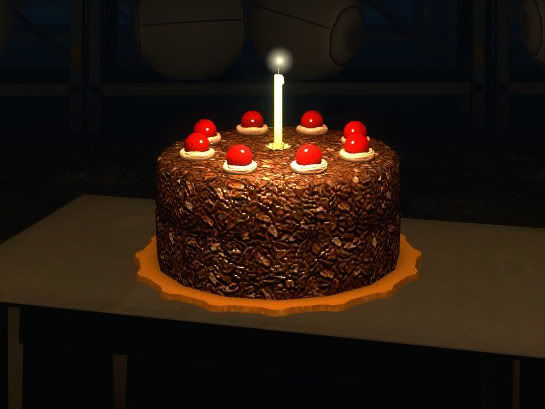
\includegraphics[width=.4\textwidth]{cake.jpg}}\\
	\end{tabular}
	\vspace{5em} 
	\vspace{3em} \hrule
	\vspace{3em} \hrule
	\vspace{3em} \hrule
	\vspace{3em} \hrule
	\vspace{3em} \hrule
	\newpage

	\section{Cake 2}
	\blindtext
	\newpage

	\section{Cake 3}
	\blindtext
	\newpage

\chapter{Cookies}
\blindtext
\newpage

	\section{Coconut Oatmeal Cookies}
	\begin{tabular}{p{.5\textwidth} r}
		\begin{itemize}
			\item 2 cups of brown sugar
			\item 2 cups of margarine or butter
			\item 3 eggs
			\item 3 cups of rolled oats
			\item \(1\frac{1}{2}\) cups of coconut
			\item 2 teaspoons of baking powder
			\item 1 teaspoon of baking soda
			\item \(\frac{1}{2}\) salt
			\item vanilla
		\end{itemize}
		& \raisebox{-\totalheight}{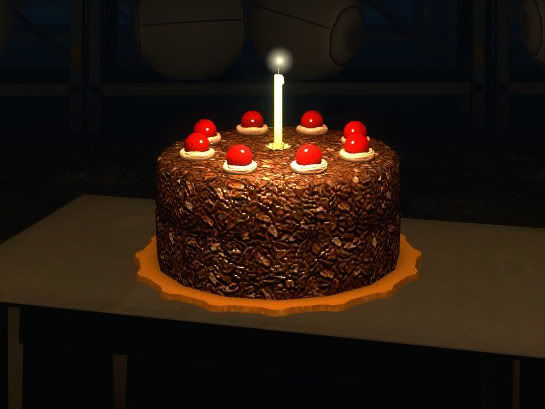
\includegraphics[width=.4\textwidth]{cake.jpg}}\\
	\end{tabular}

	\noindent
	Shape in a ball.  Press with a fork, and bake at \(350\degree\) F for 8-10 minutes.
	\vspace{3em} \hrule
	\vspace{3em} \hrule
	\vspace{3em} \hrule
	\vspace{3em} \hrule
	\vspace{3em} \hrule
	\newpage

	\section{Double Ginger Crackles}
	\begin{tabular}{p{.5\textwidth} r}
		\begin{itemize}
			\item 10 oz. \(\left(2\frac{1}{4}\text{ cups}\right)\) unbleached all-purpose flour
			\item \(2\frac{3}{4}\) teaspoons of ground ginger
			\item 1 teaspoon of baking soda
			\item \(\frac{1}{4}\) teaspoons of table salt
			\item 6 oz. \(\left(\frac{3}{4} \text{ cups}\right)\) unsalted butter, at room temperature
			\item \(1\frac{1}{3}\) cups of brown sugar
			\item 1 large egg at room temperature
			\item \(\frac{1}{4}\) cups of molasses
			\item 3 tablespoons of finely chopped crystallized ginger
		\end{itemize}
		& \raisebox{-\totalheight}{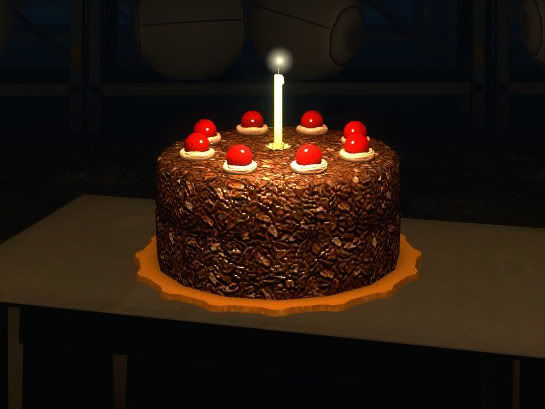
\includegraphics[width=.4\textwidth]{cake.jpg}}\\
	\end{tabular}

	\noindent
	Position racks in the upper and lower thirds of the oven and heat the oven to \(350\degree\) F.  Line two large baking sheets with parchment or nonstick baking liners.\\

	\noindent
	In a medium bowl, whisk the flour, ground ginger, baking soda, and salt.  In a large bowl, beat the butter and 1 cup of the sugar with an electric mixer (a stand mixer fitted with the paddle attachment, or a hand-held) on medium-high speed until well blended.  Add the egg, molasses, and crystallized ginger; beat well.  Add the dry ingredients and mix on low speed until well blended.\\

	\noindent
	Pour the remaining \(\frac{1}{2}\) cup of sugar into a shallow bowl.  Using a 1 tablespoon cookie scoop, a small ice cream scoop, or two tablespoons, shape the dough into 1 inch balls.  Roll each ball in the sugar to coat.  Set the balls \(1\frac{1}{2}\) to 2 inches apart on the prepared baking sheets.\\

	\noindent
	Bake, rotating the sheets halfway through, until the cookies are puffed and the bottoms are lightly browned, 12 to 14 minutes.  If you touch a cookie, it should feel dry on the surface but soft inside.  The surface cracks will look a bit wet.  Let the cookies sit on the cookie sheet for 5 minutes and then transfer them to a rack to cool completely.  When cook, store in airtight containers for up to five days.\\
	\vspace{3em} \hrule
	\vspace{3em} \hrule
	\vspace{3em} \hrule
	\vspace{3em} \hrule
	\vspace{3em} \hrule
	\newpage

\chapter{Muffins}
\blindtext
\newpage

	\section{Best Ever Basic Muffins}
	\begin{tabular}{p{.5\textwidth} r}
		\begin{itemize}
			\item 2 cups of flour
			\item \(\frac{3}{4}\) cups of white sugar
			\item \(\frac{1}{2}\) teaspoons of salt
			\item 3 teaspoons of baking powder
			\item 1 egg
			\item \(\frac{1}{2}\) cups of oil
			\item \(\frac{3}{4}\) cups of milk
		\end{itemize}
		& \raisebox{-\totalheight}{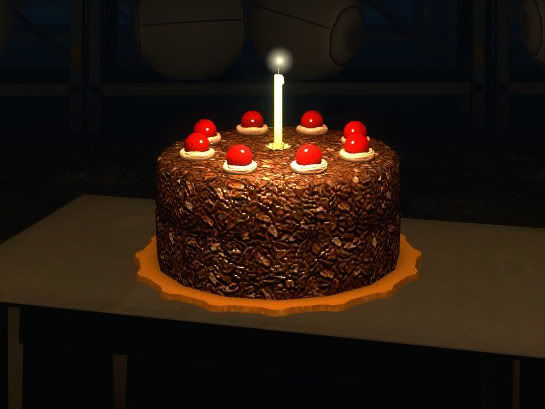
\includegraphics[width=.4\textwidth]{cake.jpg}}\\
	\end{tabular}

	\noindent
	Sift together the flour, white sugar, salt, and baking powder into a mixing bowl and mix in whatever fruit or nuts you wish.  Whisk together the egg, oil, and milk then quickly stir the liquid into the flour mix - don't over mix.  Bake at \(400\degree\) F for 20 minutes.  Makes 12 muffins.\\

	\noindent
	Try adding apples and raisins, peaches, bananas, or chopped nuts.\\

	\noindent
	For cranberry muffins use \(\frac{3}{4}\) cups of orange juice in place of the milk and add a good cup of cut cranberries.  This makes a very nice muffin.
	\vspace{3em} \hrule
	\vspace{3em} \hrule
	\vspace{3em} \hrule
	\vspace{3em} \hrule
	\vspace{3em} \hrule
	\newpage

\end{document}
